\section{Design}
\label{sec:design}

%% [Section roadmap] This section presents the hybrid defense system design: problem setting, system overview, three core modules, and deployment considerations.
In this section, we present the design of our hybrid defense system for detecting malicious behaviors embedded in model artifacts. We first formalize the problem setting and design goals of the system. Then we provide a high-level system overview and detail three core modules that jointly model (i) non-bypassable low-level system-call evidence and (ii) high-dimensional Python semantic context collected via non-invasive instrumentation. Finally, we discuss deployment considerations that enable practical and safe use in real-world analysis environments.
\begin{figure*}[!t]
    \centering
    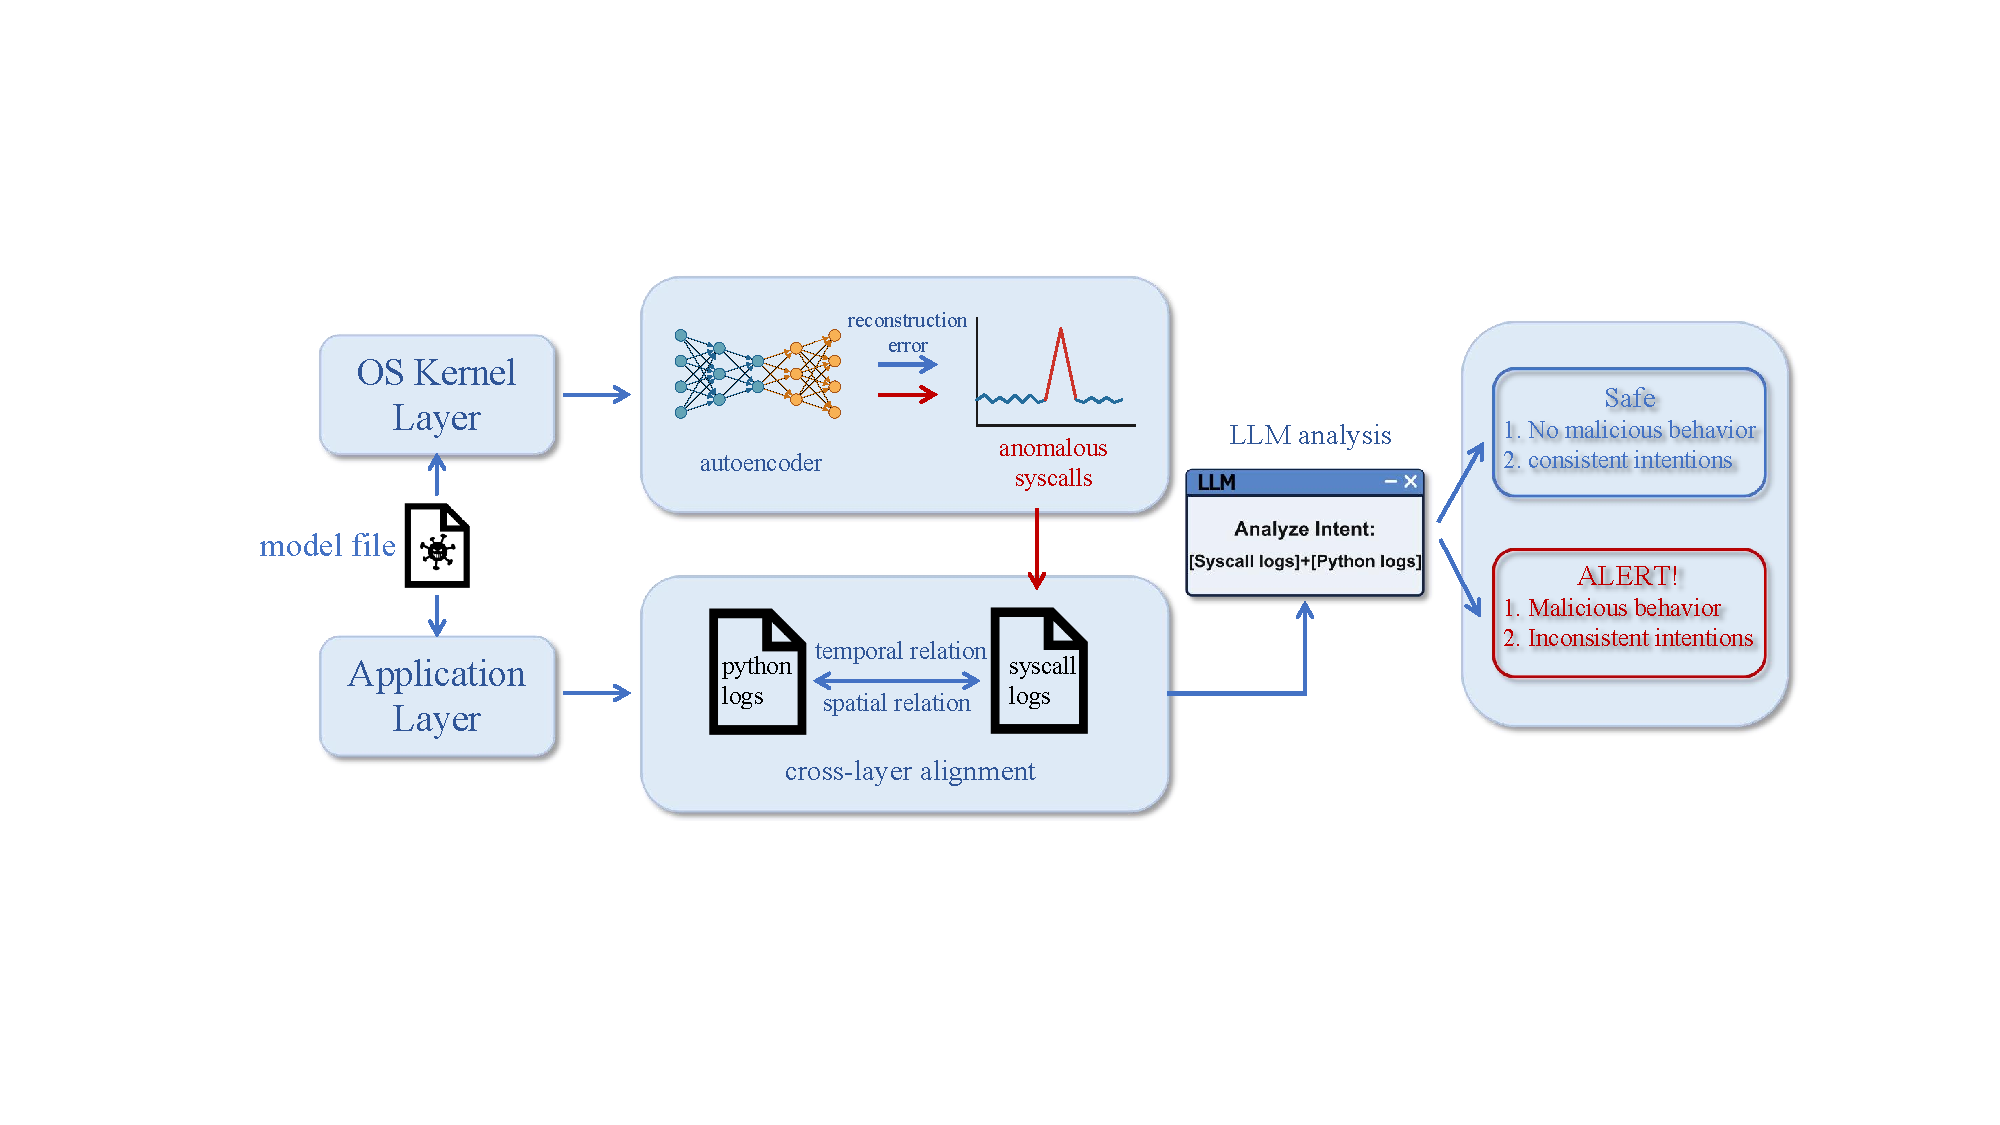
\includegraphics[width=\linewidth]{figs/overview1.pdf}
    \caption{Overview of the hybrid defense system.}
    \label{fig:overview}
\end{figure*}


\subsection{System Overview}

%% [Input definition] The system ingests a model artifact and a controlled execution configuration as its two inputs.
\noindent \textbf{Input.} 
The system takes a model artifact $M$ (e.g., a checkpoint/weights file, a serialized object, or a model package) and a controlled execution configuration $E$.

%% [Dual observation streams] Two synchronized streams are collected: Python semantic logs and kernel-level system-call traces.
\noindent \textbf{Observations.} During execution, we collect two synchronized streams:
an application-layer semantic log stream $L=\{(\ell_i,t_i)\}$ from Python instrumentation, and
a kernel-visible system-call stream $S=\{(s_j,\tau_j)\}$ from system-call tracing.

%% [Structured alert output] Each alert carries an intent score, threat category, and an evidence chain linking semantic context to low-level operations.
\noindent \textbf{Output.} The system outputs a structured alert
\begin{equation}
A = \langle \textit{IntentScore},\; \textit{ThreatCategory},\; \textit{Context} \rangle,
\end{equation}
where $\textit{IntentScore}\in[0,1]$ reflects the likelihood of malicious intent, $\textit{ThreatCategory}$ is the predicted attack type, and $\textit{Context}$ is an evidence chain linking semantic context to low-level behaviors, which contains abnormal system-call operations and aligned high-level Python semantic events.

%% [Three design goals] Non-bypassability via syscall evidence, low false positives via semantic context, and efficiency via prefiltering.
\noindent \textbf{Goals.} Our design targets three goals: (G1) \emph{non-bypassability} via system-call evidence; (G2) \emph{low false positives and explainability} via semantic context; and (G3) \emph{efficiency and deployability} via fast prefiltering and lightweight instrumentation.


%% [Module 1 summary] Kernel-level syscall aggregation and autoencoder-based prefiltering to surface suspicious operations.
\noindent \textbf{Module 1: } Kernel-level behavior extraction and prefiltering. We aggregate raw system calls into higher-level ``operations'' and use an Autoencoder to quickly identify abnormal operations. This module turns noisy, fine-grained traces into compact operation vectors and filters out clearly benign behavior, ensuring that only suspicious low-level activities are forwarded for deeper analysis.

%% [Module 2 summary] Non-invasive Python instrumentation capturing semantic context around security-relevant API calls.
\noindent \textbf{Module 2:} Application-layer semantic instrumentation. We perform non-invasive, framework-adaptive Python instrumentation to capture high-dimensional semantic context around security-relevant API calls. This module logs which libraries and APIs are invoked, with what summarized arguments and in which execution phase, providing the semantic side of the evidence chain.

%% [Module 3 summary] Cross-layer association of abnormal syscalls with semantic context, fed to an LLM for intent reasoning.
\noindent \textbf{Module 3: } Cross-layer association and LLM reasoning. We align abnormal low-level operations with nearby semantic contexts, then ask an LLM to judge whether the behavior is explainable under benign model execution, producing an intent score and an evidence chain. This module links what the model code appears to be doing with what the operating system actually observes, and converts the combined evidence into a human-understandable alert.

\subsection{Kernel-level Behavior Extraction and Prefiltering}
% The second module operates at the operating system level and is responsible for turning raw system-call traces into a small set of suspicious ``operations'' for further cross-layer analysis. Directly modeling single system calls is impractical because they are extremely fine-grained and voluminous, and because meaningful behavior  always manifests as a \emph{sequence} of related calls.
%% why we use system-call traces.
This module processes raw system-call traces captured during model execution and converts them into a compact set of suspicious ``operations'' for downstream cross-layer analysis. We base our detection on system-call traces because they operate below the user-space level and cannot be bypassed by any Python-level obfuscation\cite{2875487}: no matter how a model artifact hides its malicious intent through code mangling or dynamic loading, its actual interactions with the operating system must traverse the kernel and therefore leave a non-bypassable forensic record.  

%% [Challenge: raw syscalls are too fine-grained] 
However, directly modeling individual system calls is impractical because they are extremely fine-grained and voluminous. A single model loading process may produce tens of thousands of system calls. Moreover, meaningful malicious behavior invariably manifests as a \emph{sequence} of related calls rather than as isolated events. Accordingly, by aggregating correlated system calls into high-level operational units, this module could reduces trace noise, compresses data volume, and outputs standardized analysis units with complete semantics that facilitate subsequent anomaly detection computations.

\begin{table}[t!]
	\centering
	\caption{Security-relevant system-call categories used by our filter.}
	\begin{tabular}{l p{0.28\columnwidth} p{0.45\columnwidth}}
		\hline
		Filter param & Category & Purpose \\
		\hline
		file   & File operations (\texttt{read}/\texttt{write}) & Detect sensitive data leakage or configuration file tampering \\
		network & Network operations (\texttt{socket}) & Detect data exfiltration or remote command execution \\
		cred   & Credential operations (\texttt{setuid}) & Detect privilege-escalation behavior \\
		desc   & Descriptor operations (\texttt{dup}) & Assist file-related anomaly detection \\
		signal & Signal handling (\texttt{kill}) & Capture malicious process termination attempts \\
		clock  & Time-related operations & Assist temporal anomaly analysis (e.g., abnormal delays) \\
		\hline
	\end{tabular}
	\label{tab:syscalltypes}
\end{table}

\noindent \textbf{System-call collection and filtering.} % During controlled model execution, we use \texttt{strace} to continuously trace system calls of the target process. To reduce noise and overhead, we immediately discard high-frequency but semantically uninformative calls such as scheduler hints. The selection of system calls focuses on those that are security-relevant, ensuring that the tracing process captures meaningful behaviors while minimizing unnecessary data collection. Table~\ref{tab:syscalltypes} summarizes the security-relevant syscall families we monitor and their roles in our detection pipeline. For example, file operations can indicate attempts to access sensitive data or modify configurations, while network operations may signal data exfiltration or remote command execution. 
%% [Solution: selective tracing] Only security-relevant syscall families are traced; uninformative calls are discarded to keep trace volume manageable.
We employ a selective tracing strategy that focuses exclusively on security-relevant system-call families, discarding high-frequency but semantically uninformative calls to keep the trace volume manageable. During controlled model execution, we use \texttt{strace} to continuously trace system calls of the target process. To reduce noise and overhead, we immediately discard calls such as scheduler hints and memory-mapping operations that carry no security signal\cite{shakya2022analysisdetectionclassificationandroid}. The selection concentrates on system-call categories that can indicate malicious intent. Table~\ref{tab:syscalltypes} summarizes the security-relevant syscall families we monitor and their roles in our detection pipeline. For example, file operations can reveal attempts to access sensitive data or modify configurations, while network operations may signal data exfiltration or remote command execution.

%% [Two syscall categories] 
To accurately model the execution semantics of a program, it is crucial to recognize that system calls inherently possess varying degrees of contextual dependency. Applying a uniform extraction strategy to all system calls would be ineffective: some operations are semantically self-contained and immediately indicative of high-risk behavior, whereas others are granular, stateful operations that remain ambiguous unless analyzed as a continuous sequence. Motivated by this fundamental difference, we propose a hybrid embedding scheme that categorizes the traced system calls into two distinct streams for targeted handling: (1) \emph{Directly malicious calls} and (2) \emph{Stateful calls}. By processing these two streams individually, we ultimately synthesize them into a unified feature space for downstream analysis.
%% [Direct call embedding] Directly malicious calls are encoded via a pre-trained Bert model into fixed-dimension vectors.

\noindent \textbf{Direct call embedding.} The first category includes standalone, high-risk operations (e.g., \texttt{execve}, \texttt{chmod}) that do not require lifecycle context. We directly encode each of these calls into a fixed-dimension operation vector $\mathbf{v}_{\textit{dir}} \in \mathbb{R}^{d}$. Specifically, we utilize a pre-trained BERT-based model to extract the rich semantic meaning from the call's underlying logic and literal arguments. This high-dimensional representation is subsequently projected down to the target dimension $d$, ensuring that semantically critical, self-contained threats are instantly captured without the need for sequence aggregation.

\noindent \textbf{Stateful aggregation.} Let $S = \{(s_k, \tau_k)\}_{k=1}^{N}$ denote the traced system-call stream, where $s_k$ is the $k$-th syscall and $\tau_k$ its timestamp. For stateful operations, we maintain per-resource state keyed by $r = \langle \textit{PID}, \textit{FD} \rangle$, where $\textit{FD}$ denotes a file or socket descriptor. For each key $r$, we collect the indices of calls that operate on this resource within one lifecycle segment,
\begin{equation}
I_r = \{\, k \mid (s_k, \tau_k) \in S,\ s_k \text{ uses resource } r,\ \tau_{\textit{start}}^r \le \tau_k \le \tau_{\textit{end}}^r \,\},
\end{equation}
where $\tau_{\textit{start}}^r$ and $\tau_{\textit{end}}^r$ are the timestamps of the resource-acquisition and resource-release calls (e.g., \texttt{open} / \texttt{close} or \texttt{socket} / \texttt{shutdown}). The lifecycle segment for resource $r$ is then the ordered subsequence $S_r = \{(s_k, \tau_k)\}_{k \in I_r}$.

%% [Feature extraction from lifecycle segments] Each per-resource lifecycle segment is compressed into a fixed-length vector via lightweight statistical features.
We aggregate this segment into a fixed-length operation vector by applying a feature-extraction function $\phi$ over all calls in the segment:
\begin{equation}
\mathbf{v}_{\textit{sys}}(r) = \phi(S_r) \in \mathbb{R}^{d},
\end{equation}
where $\phi$ operates by extracting the common resource identifier $r = \langle \textit{PID}, \textit{FD} \rangle$ shared across the segment $S_r$, and concatenating it with the sequence of distinct, call-specific parameters (e.g., flags, buffer sizes, or return values) derived from each individual system call $s_k \in S_r$. This concatenated feature sequence is subsequently passed through an embedding layer to project it into the continuous $\mathbb{R}^{d}$ space. Intuitively, each $\mathbf{v}_{\textit{sys}}(r)$ captures a dense, contextualized representation of the exact data flow and state transitions associated with a specific file or connection during its lifetime, effectively smoothing out scheduling artifacts and interleaving from other threads.


%% [Hybrid feature representation] Direct and aggregated vectors are combined into a unified feature matrix capturing both immediate and contextual syscall behaviors.
The final feature matrix combines $\mathbf{v}_{\textit{dir}}$ and $\mathbf{v}_{\textit{sys}}$, enabling the system to capture both direct and aggregated syscall behaviors. This hybrid representation ensures that directly malicious actions are immediately flagged, while stateful operations are analyzed in context to detect more subtle threats.

% Both direct operations $\mathbf{v}_{\textit{dir}}$ \shaofei{what is $V_{dir}$?} and aggregated operations $\mathbf{v}_{\textit{sys}}$ are encoded as fixed-length feature vectors. The feature set includes lightweight statistics such as per-call-type counts, total bytes read and written, error-code distributions, duration of the lifecycle segment, and simple flags describing access patterns (e.g., read-only vs. write-heavy, local vs. remote destination). The exact feature schema is configurable and can be extended to cover new behaviors, but is chosen so that benign model loading and inference exhibit a stable, learnable distribution, while malicious behaviors (e.g., spawning shells or exfiltrating secrets) produce outlier vectors.
% \shaofei{also formalize this part. I think this part can be merged with the previous one. }

%% why we use unsupervised learning and why we choose an autoencoder for anomaly detection.
\noindent \textbf{Autoencoder-based anomaly detection.} We adopt unsupervised anomaly detection because benign model loading and inference produce a stable, learnable distribution of system-call operations, whereas malicious behaviors are inherently rare and diverse, making supervised classification impractical without labeled attack samples that cover the full threat space. Among unsupervised methods, we choose an Autoencoder for its conceptual simplicity and proven effectiveness in reconstruction-based anomaly detection: it learns to faithfully reconstruct benign operation vectors during training and naturally flags any vector it cannot faithfully reconstruct as anomalous.

We train an Autoencoder on operation vectors collected from clean model loading and inference runs. Given an operation vector $\mathbf{v}$, the Autoencoder computes a reconstruction error
\begin{equation}
E = \left\lVert \mathbf{v} - \textit{Dec}(\textit{Enc}(\mathbf{v})) \right\rVert_2^2,
\end{equation}
where \textit{Enc} and \textit{Dec} denote the encoder and decoder networks, respectively. Operations with reconstruction error $E$ below a threshold $\theta$ are treated as consistent with normal model behavior and are discarded. If $E > \theta$, we mark the corresponding operation as abnormal, retain its full underlying system-call segment $S'$ and metadata $\langle \textit{PID}, \textit{TID}, t_{\textit{start}}, t_{\textit{end}} \rangle$, and promote it to Module~3 for semantic association and intent reasoning.

%% [Why: efficiency] Prefiltering benign operations keeps expensive LLM reasoning off the critical path for the vast majority of activity.
By performing this unsupervised prefiltering at the operation level, the system keeps the expensive cross-layer association and LLM reasoning off the critical path for the vast majority of benign activity, while still surfacing rare, suspicious low-level behaviors that deviate from the learned distribution of normal AI model execution.


\subsection{Non-invasive Python Semantic Instrumentation}
%% [Module goal] Collect Python-level semantic context to explain why the model issues specific low-level operations, bridging the semantic gap.
The goal of this module is to collect high-dimensional Python semantic context that explains why a model issues certain low-level operations. The resulting semantic log stream is later correlated with system calls to bridge the semantic gap between model-level intent and kernel-level behavior.

%% [Challenge: heterogeneous and rapidly evolving frameworks] ML frameworks expose frequently changing APIs across PyTorch, TensorFlow, JAX, and others, making manual per-framework instrumentation labor-intensive and coverage-incomplete.
Achieving comprehensive semantic instrumentation is non-trivial.The core challenge is that heterogeneous frameworks expose frequently changing internal abstractions and public APIs, making manual instrumentation both error-prone and labor-intensive. Modifying framework source code or maintaining exhaustive API checklists incurs prohibitive engineering overhead, especially as new frameworks and versions emerge. These challenges motivate our automated, LLM-assisted instrumentation approach that adapts to any framework without hand-engineering. 

\noindent \textbf{LLM-assisted Instrumentation.} %To achieve robust and adaptive monitoring across rapidly evolving AI frameworks, we propose an automated, dynamic API discovery and patching mechanism rather than relying on statically hardcoded function lists. Directly instrumenting heterogeneous frameworks is inherently challenging because their internal abstractions and public APIs change frequently. To avoid the prohibitive overhead of modifying framework source code or maintaining exhaustive API checklists, we leverage Large Language Models to synthesize dynamic probe generation scripts. Rather than manually specifying which APIs to hook, our methodology employs runtime monkey patching. The LLM is guided to generate code that iterates over the target module's namespace at process startup, systematically identifying all public callable attributes while bypassing private or internal methods.\shaofei{this part need more details. what's your prompt? how do you select the API? how you automate the instrumentation?}
%% [Solution: automated API discovery via LLM] An LLM synthesizes dynamic probe scripts that discover and wrap all public callables at runtime, eliminating manual API list maintenance.
To achieve robust and adaptive monitoring across rapidly evolving AI frameworks, we propose an automated, dynamic API discovery and patching mechanism that eliminates the need for statically hardcoded function lists. Our approach instead leverages Large Language Models to synthesize dynamic probe generation scripts that discover and wrap security-relevant APIs at runtime. The LLM is guided to generate code that iterates over the target module's namespace at process startup, systematically identifying all public callable attributes while bypassing private or internal methods. Rather than manually specifying which APIs to hook, the methodology employs runtime monkey patching to inject logging wrappers around every discovered callable, ensuring comprehensive coverage without per-framework hand-engineering.
% \shaofei{this part need more details. what's your prompt? how do you select the API? how you automate the instrumentation?}

%% [Core mechanism: structured prompt template] A rigorously constrained prompt instructs the LLM to synthesize wrappers capturing timestamps, arguments, return types, and full call stacks in standardized JSON.
The core of our approach lies in a rigorously structured prompt template that constrains the LLM to synthesize comprehensive and safe semantic wrappers. Specifically, the prompt clarifies the security objective of detecting anomalous behaviors during model loading and execution, and imposes rigorous technical constraints to guarantee operational stability of the system. The LLM is instructed to construct wrappers that capture highly detailed execution contexts before and after the original function invocation. This context includes timestamps, operation types, argument values, return types, and the complete call stack retrieved via the \texttt{traceback} module. To facilitate automated downstream analysis, the prompt mandates that all intercepted semantic events $\ell_i$ must be serialized into a standardized JSON format.

%% [Why: version adaptivity] Regenerating wrappers for new API surfaces suffices---the core detection pipeline remains unchanged across framework versions.
The instrumentation is designed to be adaptive: when the underlying framework version changes, we only need to regenerate the wrappers for the new API surface, without changing the core detection pipeline. This enables broad coverage across diverse model frameworks while keeping manual engineering effort low.

\begin{algorithm}[t!]
\caption{Automated Dynamic Instrumentation Logic}
\label{alg:instrumentation}
\KwIn{Target library module $\mathcal{M}$ (e.g., \texttt{torch}, \texttt{tensorflow})}
\KwOut{Instrumented module capable of context logging}

\SetKwProg{Fn}{Procedure}{:}{}
\SetKwFunction{FApply}{ApplyDynamicPatches}
\SetKwFunction{FConstruct}{Wrapper}

\Fn{\FApply{$\mathcal{M}$}}{
    \ForEach{attribute name $attr\_name$ \textnormal{\textbf{in}} \textnormal{dir}($\mathcal{M}$)}{
        \If{$attr\_name$ starts with ``\_''}{
            \textbf{continue} 
        }
        
        $target\_func \gets$ \textnormal{getattr}($\mathcal{M}, attr\_name$)\;
        \If{\textnormal{\textbf{not}} is\_callable($target\_func$)}{
            \textbf{continue} 
        }
        
        $wrapper \gets$ \FConstruct{$target\_func, attr\_name$}\;
        
        \textbf{try}\;
        \Indp \textnormal{setattr}($\mathcal{M}, attr\_name, wrapper$)\; 
        \Indm \textbf{catch} \textit{ReadOnlyAttributeError} \;
        \Indp \textbf{continue} \;
        \Indm
    }
}
\Fn{\FConstruct{$func, name$}}{
    \KwRet a closure that captures the full \texttt{traceback}, logs to JSON, executes $func$, and delegates return value\;
}
\end{algorithm}

The core workflow of the instrumentation is formalized in Algorithm~\ref{alg:instrumentation}. During the \texttt{ApplyDynamicPatches} procedure, the script systematically iterates through the target module $\mathcal{M}$. After isolating the public, callable APIs, it dynamically constructs a \texttt{Wrapper} closure based on the LLM's specifications. It then employs runtime monkey patching (\texttt{setattr}) to replace the original function with our intercepted version, incorporating exception handling to safely bypass read-only or immutable attributes.

%%Each monitored API call is recorded as a structured semantic event with PID, timestamp, function name, and compact argument summary.
\noindent \textbf{Data Collection} 
Once the dynamic patches are successfully applied at startup, any invocation of the targeted APIs by the user's code or framework internals will automatically trigger the injected closures. These wrappers execute the semantic extraction logic and serialize the intercepted context into a standardized format. Consequently, each monitored API call is recorded as a structured semantic event:
\begin{equation}
\ell_i = \langle \textit{FuncName},\; \textit{ArgsSummary} \rangle.
\end{equation}
where $\textit{FuncName}$ typically corresponds to security-relevant framework or standard-library APIs. $\textit{ArgsSummary}$ aggregates only lightweight, non-sensitive information such as tensor shapes and dtypes, configuration flags, truncated or hashed file paths, and bounded-length string summaries. This design ensures that the semantic log stream $L$ captures rich contextual information about the model's execution while controlling logging overhead.

%% [Why: conservative safety policy] Wrappers are restricted to callable functions, kept thin to avoid side effects, and use defensive argument serialization to prevent runtime breakage.
\noindent \textbf{Safety constraints.} To reduce the risk of breaking runtime behavior, the instrumentation follows a conservative policy. First, we only wrap callable functions and avoid replacing class definitions, built-in data types, or objects backed by low-level C/C++ bindings. Second, wrappers are kept as thin as possible: they perform best-effort argument summarization and then immediately invoke the original function, without altering return values or side effects. Third, the parameter serialization adopts defensive strategies to control logging overhead by recording only shapes instead of raw tensor contents, truncating long strings, and other similar methods. 

% Furthermore, to preserve the original control and data flow of the ML framework, the generated script enforces graceful exception handling. Modern AI frameworks typically possess highly complex internal architectures, heavily utilizing read-only properties, immutable C-extension bindings, and dynamically generated descriptors. A naive monkey-patching approach would inevitably trigger fatal runtime errors when attempting to overwrite these restricted components, thereby crashing the process during model initialization. To mitigate this risk, our framework's prompt design constraints the LLM to wrap both the dependency injection phaseand the runtime execution phase of the generated wrappers within protective \texttt{try-except} blocks. 
%% [Why: graceful exception handling] Try-except blocks around patching protect against crashes from read-only properties and C-extension bindings, ensuring degraded rather than fatal failures.
Moreover, to preserve the original control and data flow of the ML framework, the generated instrumentation script enforces graceful exception handling throughout the patching process. Modern AI frameworks possess highly complex internal architectures that heavily utilize read-only properties, immutable C-extension bindings, and dynamically generated descriptors. A naive monkey-patching approach that attempts to overwrite these restricted components would inevitably trigger fatal runtime errors, crashing the process during model initialization. To mitigate this risk, our framework's prompt design constrains the LLM to wrap both the dependency injection phase and the runtime execution phase of the generated wrappers within protective \texttt{try-except} blocks, ensuring that any patch failure degrades without disrupting the target process.

\subsection{Cross-layer Spatio-temporal Association}
%% [Module 3 role] Receives abnormal operations from Module 1 and associates them with semantic context from Module 2 to determine whether behavior is benign.
The third module receives abnormal operations reported by Module~1 and associates them with high-dimensional Python semantic context from Module~2. Its primary goal is to determine whether each abnormal low-level operation can be reasonably explained as benign model behavior. For suspicious operations that cannot be justified as benign, we further construct a complete cross-layer behavior profile to locate the model code triggering such behaviors and analyze their potential maliciousness.

%% [Challenge: asynchrony between syscalls and Python semantics] OS scheduling and concurrent I/O make naive timestamp matching unreliable; a fuzzy spatio-temporal strategy is needed.
System calls and Python semantics are inherently asynchronous due to operation system scheduling and concurrent I/O. As a result, naive one-to-one timestamp matching between logs $S$ and $L$ is unreliable in high-concurrency workloads. We therefore adopt a fuzzy spatio-temporal association strategy.

%% 
For each abnormal operation, Module~1 provides the underlying system-call segment $S'$ and its metadata $\langle \textit{PID}, t_{\textit{start}}, t_{\textit{end}} \rangle$. Given this metadata and the semantic log stream $L = \{(\ell_i, t_i)\}$, Module~3 performs filtering following the spatial-temporal matching rules below.

%% [Step 2: temporal windowing] A slack time window around the operation's lifespan captures semantic events with tolerance for scheduling jitter.
\noindent \textbf{Temporal windowing.} We then apply a slack temporal window around the abnormal operation. For each candidate abnormal operation, we define its active time span $[t_{\textit{start}}, t_{\textit{end}}]$ based on the first and last system call in $S'$, and search semantic events whose timestamps $t_i$ fall into an expanded window $[t_{\textit{start}} - \Delta t, t_{\textit{end}} + \Delta t]$. The slack parameter $\Delta t$ tolerates minor scheduling jitter while still localizing semantic context to the period when the resource was actually in use.

%% [Step 3: spatial hints disambiguate concurrency] Resource-derived hints (file paths, network destinations) further filter candidates when temporal proximity alone is insufficient.
\noindent \textbf{Spatial hints.} Temporal proximity alone is insufficient under heavy concurrency. We therefore further filter candidates using resource-related hints derived from both layers, such as whether the operation is file- or network-related, file paths or prefixes, remote destinations, and other descriptor metadata when available. Combining temporal and spatial constraints yields a fuzzy but robust alignment that significantly reduces spurious associations when many model components execute in parallel.

%% [Output: cross-layer behavior profile] Filtered evidence is bundled into a structured profile containing OS observations, Python API context, and execution-phase information for LLM reasoning.
\noindent \textbf{Cross-layer behavior profile.} After spatio-temporal filtering, Module~3 bundles the abnormal operation vector, its raw system-call summary, and the aligned semantic events into a structured cross-layer behavior profile. This profile serves as the input to the LLM-based intent reasoning stage: it contains (i) what the OS observed at the system-call level, (ii) which high-level Python APIs and call sites were active around that time and on the same resource, and (iii) basic execution-phase information. Together, these elements provide sufficient context to decide whether the abnormal low-level behavior is consistent with benign model execution or indicative of malicious intent.

\subsection{LLM-based Intent Reasoning and Evidence Chain Generation}
%% [Challenge: intent ambiguity] The same syscall pattern can arise from legitimate model loading or malicious exfiltration; the LLM resolves this ambiguity by jointly analyzing low-level and semantic evidence.
Determining whether abnormal low-level operations reflect benign model behavior or malicious intent is inherently challenging: the same system-call pattern can arise from legitimate model loading or from an attacker's attempt to exfiltrate data, and without semantic context the two are indistinguishable at the kernel level. To resolve this ambiguity, we feed each abnormal operation together with its aligned semantic contexts into an LLM, which judges whether the behavior is consistent with benign model execution.

%% [Prompt design] The aligned evidence is translated into a natural-language prompt summarizing the operation, its semantic context, and the execution phase.
\noindent \textbf{Prompt construction.} We translate the aligned evidence into a structured natural-language prompt that includes: (i) a concise summary of the abnormal operation including operation type, key statistics, and risk-relevant parameters, (ii) the aligned semantic call contexts including library/API, call stack summary, and argument summaries, and (iii) the execution phase categorized into the model loading stage and inference stage.

%% the last part of prompt is how to estimate malicious: If malicious-looking behaviors in system calls can be reasonably interpreted as legitimate business behaviors via Python-level instrumentation semantics, such behaviors are deemed benign. In cases where inconsistencies exist between Python-layer semantic logs and corresponding system call activities, or no matching Python semantic context can be retrieved to justify the system call, the concerned behavior is marked malicious.
Our maliciousness judgment follows a principled cross-layer reasoning rule: a behavior is classified as benign only when its low-level system-call activity can be plausibly explained by the aligned Python-level semantic context. Concretely, if the LLM identifies that the observed file reads, network connections, or process creations are consistent with the framework APIs and execution phase reported in the semantic log, the operation is deemed benign and discarded. Conversely, when inconsistencies exist between the Python-layer semantic logs and the corresponding system-call activities, such as a network connection to an external host with no matching high-level API invocation, or when no matching Python semantic context can be retrieved at all, the behavior is marked as malicious and escalated.


%% [LLM output: score, category, evidence chain] The LLM returns an intent score and threat category, with the reasoning inputs persisted as an auditable evidence chain.
\noindent \textbf{Decision and explanation.} The LLM outputs $\textit{IntentScore}$, a $\textit{ThreatCategory}$ label, and a rationale. Importantly, we persist the subset of semantic events and system-call summaries used in the reasoning as the \emph{evidence chain} $\textit{Context}$ for auditing.

%% [Fail-safe: unexplainable high-risk patterns] System-call patterns with no matching semantic context trigger high-severity alerts and optional execution blocking.
\noindent \textbf{Fail-safe behavior.} If high-risk system-call patterns appear without any plausible semantic explanation (e.g., sensitive network connection with no corresponding high-level network API context), the system raises a high-severity alert and can optionally block execution in the controlled environment.

\subsection{Deployment Considerations}
%% [Controlled sandbox execution] Analysis runs in a least-privilege environment with optional network isolation to contain confirmed malicious behaviors.
\noindent \textbf{Controlled execution.} The design assumes model analysis runs in a controlled environment with least privilege and optional network isolation, so that confirmed malicious behaviors can be contained.

%% [Extensible architecture] Instrumentation templates and operation features can be expanded for new frameworks and behaviors without pipeline changes.
\noindent \textbf{Extensibility.} The instrumentation templates can be expanded as new framework APIs emerge; similarly, operation features can be extended to cover new low-level behaviors without changing the overall pipeline.
